\documentclass[a4paper,openany]{book}
\usepackage{amssymb,amsthm,makeidx,enumerate}
\usepackage[utf8]{vietnam}
\usepackage{scrextend} %Tăng cỡ chữ
\changefontsizes{13pt}%Cỡ chữ mới là 13pt
\usepackage{times}
\usepackage{amsmath}
\usepackage{tikz}
\usepackage{enumitem}
\usepackage{array}
\usepackage[utf8]{inputenc}
\usepackage{pgfplots}
\usepackage{setspace}
\usepackage{caption}  % Gói lệnh cho phần chú thích của hình vẽ
\usepackage{tocloft}  % Gói lệnh cho chỉ mục
\usepackage[top=3.5cm, bottom=3cm, left=3.5cm, right=2cm] {geometry}
\setstretch{1.5}
\usetikzlibrary{arrows}
\makeindex
\begin{document}
\input def
\pagestyle{empty}
\begin{center}
\fontsize{14}{16}\selectfont
{ĐẠI HỌC QUỐC GIA TP. HỒ CHÍ MINH}\\
{TRƯỜNG ĐẠI HỌC KHOA HỌC TỰ NHIÊN}\\

\hfill

\vspace*{2cm}

\fontsize{14}{16}\selectfont
{\bf  PHẠM THỊ HOÀ}\\
{NGÀNH LÝ THUYẾT XÁC SUẤT VÀ THỐNG KÊ TOÁN HỌC}

\vspace*{3cm}
\fontsize{20}{22}\selectfont
{TIỂU LUẬN CUỐI KÌ }

\vspace*{1cm}
\fontsize{20}{22}\selectfont
{\bf PHƯƠNG PHÁP NGUYÊN CỨU KHOA HỌC}

\vspace*{3cm}
\fontsize{13}{16}\selectfont
GIẢNG VIÊN ĐÁNH GIÁ\\
GS.TS. BÙI XUÂN HẢI



\vfill
\fontsize{12}{16}\selectfont
{Tp. Hồ Chí Minh - 2024}
\end{center}


\newpage
\thispagestyle{empty}
\begin{center}
\fontsize{13}{16}\selectfont
{ĐẠI HỌC QUỐC GIA TP. HỒ CHÍ MINH}\\
{\bf TRƯỜNG ĐẠI HỌC KHOA HỌC TỰ NHIÊN}

\vspace*{1.5cm}
\fontsize{14}{16}\selectfont
{PHẠM THỊ HOÀ}

\vspace*{1.5cm}
\fontsize{16}{16}\selectfont
{\bf THỰC HÀNH THIẾT KẾ LUẬN VĂN BẰNG \LaTeX}

\vspace*{1.5cm}
\fontsize{13}{16}\selectfont
% {\bf LUẬN VĂN THẠC SĨ}\\[20pt]
NGÀNH: LÝ THUYẾT XÁC SUẤT VÀ THỐNG KÊ TOÁN HỌC\\[10pt]
Mã số Ngành: 8460106

\vspace*{3cm}

NGƯỜI HƯỚNG DẪN KHOA HỌC

{TS. TRỊNH THANH ĐÈO}

\vfill
\fontsize{13}{16}\selectfont
{Tp. Hồ Chí Minh - 2024}
\end{center}


\vspace*{3cm}

\begin{center}
\LARGE{\textbf{Lời cam đoan}}
\end{center}

Tôi, Phạm Thị Hoà, cam đoan rằng luận văn này là công trình nghiên cứu của riêng tôi dưới sự hướng dẫn của TS.Trịnh Thanh Đèo. Tất cả các nguồn tài liệu và thông tin tham khảo đã được ghi rõ và được sử dụng một cách công bằng và trung thực.

Tôi xin cam đoan rằng tất cả các phần của luận văn này được viết bởi chính tôi và không sao chép từ bất kỳ nguồn nào khác mà không được ghi chú rõ ràng.


\begin{flushright}
{\it Tp.HCM, ngày 30 tháng 05 năm 2024}

Tác giả\hskip 2cm\quad

\vskip 2cm

{\bf Phạm Thị Hoà} \hskip 1cm \quad\ 
 \end{flushright}
\thispagestyle{empty}

% \vspace*{3cm}

\begin{center}
\LARGE{\textbf{Lời cảm ơn}}
\end{center}

Tôi xin gửi lời cảm ơn chân thành và sâu sắc nhất đến những người đã góp phần làm nên sự thành công của luận văn này.

Đầu tiên, tôi muốn bày tỏ lòng biết ơn sâu sắc đến Thầy TS. Trịnh Thanh Đèo, người đã dành thời gian và kiến thức để hướng dẫn và động viên tôi trong suốt quá trình nghiên cứu. Sự hỗ trợ và sự phản hồi chân thành từ Thầy không chỉ giúp tôi hoàn thành luận văn mà còn là nguồn động viên lớn lao trong hành trình học tập của tôi.

Tôi không thể không nhắc đến gia đình và bạn bè, những người đã luôn ở bên cạnh và động viên tôi trong suốt thời gian này. Sự ủng hộ vô điều kiện của họ đã giúp tôi vượt qua những thử thách và trở thành người tốt hơn.

Cuối cùng, tôi muốn gửi lời cảm ơn đến tất cả những người đã đọc và đánh giá luận văn này. Sự quan tâm và nhận xét của các bạn là động lực lớn lao giúp tôi hoàn thiện hơn.
\begin{flushright}
{\it Tp.HCM, ngày 30 tháng 05 năm 2025}

Tác giả\hskip 2cm\quad

\vskip 2cm

{\bf Phạm Thị Hoà} \hskip 1cm \quad\ 
 \end{flushright}
\thispagestyle{empty}

\tableofcontents
\addcontentsline{toc}{chapter}{\listfigurename}
\listoffigures
\begin{titlepage}
\begin{center}
    {\bf TRANG THÔNG TIN LUẬN VĂN}
\end{center}
\addcontentsline{toc}{chapter}{Trang thông tin luận văn}
\author{}
\date{}
% \maketitle

Tên đề tài luận văn: THỰC HÀNH THIẾT KẾ LUẬN VĂN BẰNG \LaTeXe

Ngành: Lý thuyết xác suất và thống kê toán học

Mã số ngành: 8460106

Họ tên học viên cao học: Phạm Thị Hoà

Khóa đào tạo: 2023-2025

Người hướng dẫn khoa học: TS. Trịnh Thanh Đèo

Cơ sở đào tạo: Trường Đại học Khoa học Tự nhiên, ĐHQG.HCM


{\bf 1. TÓM TẮT NỘI DUNG LUẬN VĂN:}
\begin{itemize}[label=-]
    \item Giới thiệu về mô hình nhân tố trực giao và vai trò của nó trong phân tích dữ liệu.
    \item Giới thiệu về chương trình hình học lớp 12 với nội dung thể tích của hình lăng trụ và hình chóp.
\end{itemize}


{\bf 2. NHỮNG KẾT QUẢ MỚI CỦA LUẬN VĂN:}

\vspace*{1cm}

{\bf 3. CÁC ỨNG DỤNG/ KHẢ NĂNG ỨNG DỤNG TRONG THỰC TIỄN HAY NHỮNG VẤN ĐỀ CÒN BỎ NGỎ CẦN TIẾP TỤC NGHIÊN CỨU}
\vspace*{1cm}

\begin{tabular}{>{\centering\arraybackslash}m{5cm} >{\centering\arraybackslash}m{5cm} >{\centering\arraybackslash}m{5cm}}
    {\bf TẬP THỂ CÁN BỘ HƯỚNG DẪN} & & {\bf HỌC VIÊN CAO HỌC} \\
    (Ký tên, họ tên) & & (Ký tên, họ tên) \\
    & & \\
    & & \\
    & & \\
    & & \\
    & & \\
    & & \\
    & & \\
    & & \\
    & & \\
    \multicolumn{3}{c}{\bf XÁC NHẬN CỦA CƠ SỞ ĐÀO TẠO} \\
    \multicolumn{3}{c}{\bf HIỆU TRƯỞNG} \\
\end{tabular}
\end{titlepage}
\chapter*{Lời nói đầu}
\addcontentsline{toc}{chapter}{Lời nói đầu}

Trong thời đại số hóa và phát triển khoa học kỹ thuật, việc nghiên cứu và ứng dụng các phương pháp thống kê và mô hình hóa dữ liệu đang trở nên ngày càng phổ biến và quan trọng. Một trong những phương pháp mạnh mẽ được áp dụng trong nghiên cứu về dữ liệu đa biến là mô hình nhân tố trực giao.

Mặt khác chương trình hình học lớp 12 là một phần quan trọng trong chương trình giáo dục phổ thông, giúp học sinh hiểu biết và ứng dụng các kiến thức về hình học vào thực tế cuộc sống. Trong chương này, chúng ta sẽ tập trung vào việc nghiên cứu và hiểu biết về thể tích của hai hình khối quan trọng: lăng trụ và chóp.

Nội dung luận văn bao gồm 2 chương:

\begin{description}
\item [Chương 1:] Chương 1 của luận văn sẽ cung cấp một cái nhìn tổng quan về mô hình nhân tố trực giao, bao gồm cơ sở lý thuyết, các bước thực hiện và ứng dụng trong nghiên cứu. Chúng tôi sẽ giải thích cách mà mô hình này hoạt động và lý do tại sao nó được coi là một công cụ hữu ích trong phân tích dữ liệu đa biến.
\item [Chương 2:] 
Chương 2 này sẽ giới thiệu về thể tích của khối lăng trụ và khối chóp, hai khái niệm cơ bản và quan trọng trong hình học không gian. Chúng ta sẽ khám phá cách tính toán thể tích của chúng trong các bài toán thực tế.
\end{description}


\chapter{Mô hình nhân tố trực giao}
%\addcontentsline{toc}{chapter}{Chương 0. Kiến thức chuẩn bị}

\section{Giới thiệu mô hình nhân tố trực giao}

Chương 1 của luận văn trình bày về mô hình nhân tố trực giao, một phương pháp phân tích dữ liệu phổ biến trong thống kê và khoa học dữ liệu. Đầu tiên, chúng ta sẽ tổng quan về hướng nghiên cứu và mô tả các kết quả đạt được.

Hướng nghiên cứu này tập trung vào phân tích mô hình nhân tố để giải thích mối quan hệ giữa các biến quan sát và các nhân tố không quan sát được. Mục tiêu là xác định cấu trúc ẩn trong dữ liệu, giúp hiểu rõ hơn về mối quan hệ giữa các biến và nhận biết các yếu tố ẩn đằng sau chúng.

% Mô hình nhân tố được mô tả bằng một hệ phương trình tuyến tính, trong đó các biến quan sát được (X) được giả định phụ thuộc tuyến tính vào các nhân tố không quan sát được (F) và sai số (ε). Mỗi biến quan sát được biểu diễn dưới dạng một hàm tuyến tính của các nhân tố không quan sát được cộng với sai số.

Mô hình nhân tố trực giao giả định rằng các nhân tố không quan sát được độc lập và có phương sai đồng nhất. Điều này đồng nghĩa với việc mỗi nhân tố không quan sát được đều không ảnh hưởng đến nhau và có phương sai bằng nhau. Các giả định này tạo ra một mô hình đơn giản và dễ kiểm tra.

Kết quả đạt được của phần này bao gồm việc mô tả về cấu trúc mô hình nhân tố trực giao, các phương pháp ước lượng tham số mô hình, và các kỹ thuật kiểm định giả định. Thông qua các phương pháp thống kê, chúng ta có thể kiểm tra mô hình nhân tố trực giao và đánh giá mức độ phù hợp của nó với dữ liệu thực tế.

\section{Xây dựng mô hình nhân tố trực giao}

Vector ngẫu nhiên \(X\) được quan sát với các giá trị:
\begin{itemize}
\item Số thành phần: \(p\) ,
\item Trung bình: \(\mu\),
\item Ma trận hiệp phương sai: \(\Sigma\).
\end{itemize}
Mô hình nhân tố giả định rằng: \(X\) phụ thuộc tuyến tính vào một số lượng ít các nhân tố không quan sát được:
\begin{itemize}
\item \(F_1, F_2, \ldots, F_m\), được gọi là nhân tố chung (common factors).
\item \(p\) sai số  \(\boldsymbol{\epsilon}_1, \boldsymbol{\epsilon}_2, \ldots, \boldsymbol{\epsilon}_p\).
\end{itemize}
Mô hình phân tích nhân tố được mô tả:
\begin{eqnarray}
X_1 - \mu_1 &= \ell_{11}F_1 + \ell_{12}F_2 + \ldots + \ell_{1m}F_m + \boldsymbol{\epsilon}_1\\
X_2 - \mu_2 &= \ell_{21}F_1 + \ell_{22}F_2 + \ldots + \ell_{2m}F_m + \boldsymbol{\epsilon}_2
\end{eqnarray}
\[\vdots\]
\begin{eqnarray}
X_p - \mu_p &= \ell_{p1}F_1 + \ell_{p2}F_2 + \ldots + \ell_{pm}F_m + \boldsymbol{\epsilon}_p
\end{eqnarray}
hoặc, dưới dạng ký hiệu ma trận:
\begin{eqnarray}
\mathbf{X} - \boldsymbol{\mu} = \mathbf{L}\mathbf{F} + \boldsymbol{\varepsilon}
\end{eqnarray}
Trong đó: \(\ell_{ij}\) được gọi là hệ số tải (loading) của biến thứ \(i\) trên nhân tố thứ \(j\), do đó ma trận \(L\) là ma trận của các hệ số tải nhân tố (matrix of factor loadings).
Lưu ý: 
\begin{itemize}
    \item Sai số thứ \(i\) \(\boldsymbol{\epsilon}_i\) chỉ liên quan đến phản hồi \(X_i\).
    \item \(p\) độ lệch : \(X_1 - \mu_1, X_2 - \mu_2, \ldots, X_p - \mu_p\) được biểu diễn bằng \(p + m\) theo các biến ngẫu nhiên  \(F_1, F_2, \ldots, F_m, \boldsymbol{\epsilon}_1, \boldsymbol{\epsilon}_2, \ldots, \boldsymbol{\epsilon}_p\), với \(F_i\) và \(\boldsymbol{\epsilon}_i\) không thể quan sát được.
\end{itemize}

Với rất nhiều đại lượng không quan sát được, việc xác minh trực tiếp mô hình nhân tố từ các quan sát trên \(X_1, X_2, \ldots, X_p\) là không thể. Tuy nhiên, với một số giả định bổ sung về các vector ngẫu nhiên \(F\) và \(\varepsilon\), mô hình nhân tố trực giao đưa ra một số mối quan hệ hiệp phương sai, mà có thể được kiểm tra.

Chúng ta giả định rằng:
\begin{eqnarray}
E(\mathbf{F}) = \mathbf{0}_{m \times 1}, \quad \text{Cov}(\mathbf{F}) = E[\mathbf{FF}'] = \mathbf{I}_{m \times m},
\end{eqnarray}
\begin{eqnarray}
E(\boldsymbol{\varepsilon}) = \mathbf{0}_{p \times 1}, \quad \text{Cov}(\boldsymbol{\varepsilon}) = E[\boldsymbol{\varepsilon} \boldsymbol{\varepsilon}'] = \boldsymbol{\Psi} =
\begin{bmatrix}
\psi_1 & 0 & \cdots & 0 \\
0 & \psi_2 & \cdots & 0 \\
\vdots & \vdots & \ddots & \vdots \\
0 & 0 & \cdots & \psi_p
\end{bmatrix}_{p \times p},
\end{eqnarray}

Trong đó \(\mathbf{0}_{m \times 1}\) và \(\mathbf{0}_{p \times 1}\) là các vector không, \(\mathbf{I}_{m \times m}\) là ma trận đơn vị kích thước \(m \times m\), và \(\boldsymbol{\Psi}\) là ma trận đường chéo với các phần tử \(\psi_1, \psi_2, \ldots, \psi_p\) trên đường chéo chính.

Do \(F\) và \(\boldsymbol{\epsilon}\) là độc lập, vì vậy:

\begin{eqnarray}
\text{Cov}(\boldsymbol{\epsilon}, \mathbf{F}) = E(\boldsymbol{\epsilon}\mathbf{F}') = \mathbf{0}_{p \times m},
\end{eqnarray}

Những giả định này và mối quan hệ trong công thức (1.4) tạo thành mô hình nhân tố trực giao (orthogonal factor model).

\section{Ý nghĩa của mô hình nhân tố trực giao}
Trong nghiên cứu này, chúng ta đã thành công trong việc áp dụng mô hình nhân tố trực giao để phân tích mối quan hệ giữa các biến quan sát và các nhân tố không quan sát được trong một tập dữ liệu. Các kết quả chính sau đây đã được đạt được:

\begin{enumerate}
    \item Xác định cấu trúc ẩn: Mô hình nhân tố trực giao đã giúp chúng ta xác định và mô tả cấu trúc ẩn trong dữ liệu, qua đó hiểu rõ hơn về mối quan hệ giữa các biến và nhận biết các yếu tố ẩn đằng sau chúng.
    \item Đánh giá mức độ phù hợp của mô hình: Chúng ta đã sử dụng các phương pháp thống kê để kiểm tra mức độ phù hợp của mô hình với dữ liệu thực tế. Các kết quả kiểm định cho thấy rằng mô hình nhân tố trực giao có khả năng giải thích một phần lớn sự biến động trong dữ liệu.
    \item Tính giảm chiều dữ liệu: Mô hình nhân tố trực giao đã giúp chúng ta giảm chiều dữ liệu bằng cách biểu diễn các biến quan sát được dưới dạng của một số lượng ít các nhân tố không quan sát được, từ đó giúp tăng hiệu suất và khả năng hiểu quả của phân tích.
\end{enumerate}

Tóm lại, nghiên cứu này đã minh họa sự ứng dụng hiệu quả của mô hình nhân tố trực giao trong phân tích dữ liệu, đặc biệt trong việc xác định cấu trúc ẩn và giảm chiều dữ liệu. Các kết quả này có thể cung cấp sự hỗ trợ quan trọng cho quyết định và dự đoán trong nhiều lĩnh vực, từ nghiên cứu khoa học đến ứng dụng thương mại.


\chapter{Hình học}
\section{Ý nghĩa}

Hình học thể tích khối lăng trụ là một phần quan trọng trong chương trình hình học lớp 12 vì nó cung cấp kiến thức về cách tính toán và ứng dụng thể tích của các hình khối phổ biến trong thực tế. Ý nghĩa của việc nghiên cứu về thể tích khối lăng trụ trong nội dung hình học lớp 12 có thể được tóm tắt như sau:

\begin{enumerate}
    \item \textbf{Hiểu biết về không gian ba chiều:} Việc học về thể tích khối lăng trụ giúp học sinh hiểu về không gian ba chiều và cách tính toán thể tích của các hình khối phức tạp. Điều này giúp họ phát triển khả năng tư duy không gian và trực quan hóa về cách các hình khối tồn tại và tương tác trong không gian.
    
    \item \textbf{Ứng dụng trong thực tế:} Kiến thức về thể tích khối lăng trụ được áp dụng rộng rãi trong thực tế, từ xây dựng và kiến trúc đến sản xuất và logistics. Việc biết cách tính toán và đo lường thể tích của các hình khối giúp trong việc thiết kế và quản lý không gian, vật liệu và tài nguyên.
    
    \item \textbf{Phát triển kỹ năng giải quyết vấn đề:} Quá trình giải các bài toán liên quan đến thể tích khối lăng trụ yêu cầu học sinh phải áp dụng các kiến thức về hình học, đại số và tính toán. Điều này giúp họ phát triển kỹ năng giải quyết vấn đề và logic, hai kỹ năng quan trọng trong học tập và cuộc sống hàng ngày.
    
    \item \textbf{Chuẩn bị cho học tập và nghề nghiệp sau này:} Kiến thức về thể tích khối lăng trụ là một phần quan trọng của hình học và các môn học liên quan, như toán, vật lý và kỹ thuật. Việc nắm vững các khái niệm và kỹ năng này là cơ sở cho việc học tập tiếp theo và cho sự nghiệp trong các lĩnh vực liên quan đến khoa học và công nghệ.
\end{enumerate}

Vì vậy, nắm vững kiến thức về thể tích khối lăng trụ không chỉ là một yêu cầu trong chương trình hình học lớp 12 mà còn mang lại nhiều lợi ích trong việc hiểu biết thế giới xung quanh và phát triển kỹ năng sống cho học sinh.


\section{Thể tích khối lăng trụ}

Nếu ta xem khối hộp chữ nhật $ABCD.A'B'C'D'$ như là khối lăng trụ có đáy là hình chữ nhật $A'B'C'D'$ và đường cao $AA'$ thì thể tích của nó bằng diện tích đáy nhân với chiều cao. Ta có thể chứng minh được rằng điều đó cũng đúng đối với một khối lăng trụ bất kì.

Thể tích khối lăng trụ có diện tích đáy $B$ và chiều cao $h$ là:
\begin{eqnarray}
    V = Bh
\end{eqnarray}

\definecolor{aqaqaq}{rgb}{0.6274509803921569,0.6274509803921569,0.6274509803921569}
\begin{tikzpicture}[line cap=round,line join=round,>=triangle 45,x=0.3cm,y=0.3cm]
% \clip(-34.46178,-21.823355714077497) rectangle (23.554536323184955,26.839702526695376);
% \fill[line width=2.pt,color=aqaqaq,fill=aqaqaq,fill opacity=0.5] (-22.,-6.) -- (-26.,-8.) -- (-14.,-8.) -- (-10.,-6.) -- cycle;
% \fill[line width=2.pt,color=aqaqaq,fill=aqaqaq,fill opacity=0.75] (8.,-2.) -- (2.,-6.) -- (4.,-8.) -- (10.,-6.) -- (12.,-4.) -- cycle;
\draw [line width=1.2pt] (-22.,4.)-- (-26.,2.);
\draw [line width=1.2pt] (-26.,2.)-- (-14.,2.);
\draw [line width=1.2pt] (-14.,2.)-- (-10.,4.);
\draw [line width=1.2pt] (-10.,4.)-- (-22.,4.);
\draw [line width=1.2pt,dash pattern=on 5pt off 5pt] (-22.,-6.)-- (-26.,-8.);
\draw [line width=1.2pt] (-26.,-8.)-- (-14.,-8.);
\draw [line width=1.2pt] (-14.,-8.)-- (-10.,-6.);
\draw [line width=1.2pt,dash pattern=on 5pt off 5pt] (-10.,-6.)-- (-22.,-6.);
\draw [line width=1.2pt,dash pattern=on 5pt off 5pt] (-22.,4.)-- (-22.,-6.);
\draw [line width=1.2pt] (-26.,2.)-- (-26.,-8.);
\draw [line width=1.2pt] (-14.,2.)-- (-14.,-8.);
\draw [line width=1.2pt] (-10.,4.)-- (-10.,-6.);
\draw [line width=2.pt,color=aqaqaq] (-22.,-6.)-- (-26.,-8.);
\draw [line width=2.pt,color=aqaqaq] (-26.,-8.)-- (-14.,-8.);
\draw [line width=2.pt,color=aqaqaq] (-14.,-8.)-- (-10.,-6.);
\draw [line width=2.pt,color=aqaqaq] (-10.,-6.)-- (-22.,-6.);
\draw [line width=1.2pt] (4.,4.)-- (6.,2.);
\draw [line width=1.2pt] (6.,2.)-- (12.,4.);
\draw [line width=1.2pt] (12.,4.)-- (14.,6.);
\draw [line width=1.2pt] (14.,6.)-- (10.,8.);
\draw [line width=1.2pt] (10.,8.)-- (4.,4.);
\draw [line width=1.2pt] (4.,4.)-- (2.,-6.);
\draw [line width=1.2pt] (2.,-6.)-- (4.,-8.);
\draw [line width=1.2pt] (4.,-8.)-- (6.,2.);
\draw [line width=1.2pt] (12.,4.)-- (10.,-6.);
\draw [line width=1.2pt] (10.,-6.)-- (4.,-8.);
\draw [line width=1.2pt] (14.,6.)-- (12.,-4.);
\draw [line width=1.2pt] (12.,-4.)-- (10.,-6.);
\draw [line width=1.2pt,dash pattern=on 5pt off 5pt] (12.,-4.)-- (8.,-2.);
\draw [line width=1.2pt,dash pattern=on 5pt off 5pt] (8.,-2.)-- (2.,-6.);
\draw [line width=1.2pt,dash pattern=on 5pt off 5pt] (10.,8.)-- (8.,-2.);
\draw [line width=1.2pt,dash pattern=on 5pt off 5pt] (6.,2.)-- (6.,-6.);
\draw [line width=2.pt,color=aqaqaq] (8.,-2.)-- (2.,-6.);
\draw [line width=2.pt,color=aqaqaq] (2.,-6.)-- (4.,-8.);
\draw [line width=2.pt,color=aqaqaq] (4.,-8.)-- (10.,-6.);
\draw [line width=2.pt,color=aqaqaq] (10.,-6.)-- (12.,-4.);
\draw [line width=2.pt,color=aqaqaq] (12.,-4.)-- (8.,-2.);
\begin{scriptsize}
\draw [fill=black] (-22.,4.) circle (0.5pt);
\draw[color=black] (-21.511125397981257,4.699319173870623) node {$A$};
\draw [fill=black] (-26.,2.) circle (0.5pt);
\draw[color=black] (-25.631788225896308,3.5219871196583754) node {$B$};
\draw [fill=black] (-14.,2.) circle (0.5pt);
\draw[color=black] (-14.381724632223468,3.325765110623001) node {$C$};
\draw [fill=black] (-10.,4.) circle (0.5pt);
\draw[color=black] (-9.541580993085153,4.699319173870623) node {$D$};
\draw [fill=black] (-22.,-6.) circle (0.5pt);
\draw[color=black] (-20.98786662618252,-4.7847445961724775) node {$A'$};
\draw [fill=black] (-26.,-8.) circle (0.5pt);
\draw[color=black] (-26.87452780891831,-7.662667395357969) node {$B'$};
\draw [fill=black] (-14.,-8.) circle (0.5pt);
\draw[color=black] (-12.22328219855368,-7.989704077083594) node {$C'$};
\draw [fill=black] (-10.,-6.) circle (0.5pt);
\draw[color=black] (-9.083729567761258,-4.653929923482228) node {$D'$};
\draw [fill=black] (4.,4.) circle (0.5pt);
\draw[color=black] (3.670702994832952,5.418799873666996) node {$E$};
\draw [fill=black] (6.,2.) circle (0.5pt);
\draw[color=black] (6.41781154677632,3.1949504379327514) node {$F$};
\draw [fill=black] (12.,4.) circle (0.5pt);
\draw[color=black] (10.865511107065583,5.0917631919413715) node {$G$};
\draw [fill=black] (14.,6.) circle (0.5pt);
\draw[color=black] (14.462915163181899,6.661539264224367) node {$H$};
\draw [fill=black] (10.,8.) circle (0.5pt);
\draw[color=black] (7.595143783323477,9.604869399754985) node {$I$};
\draw [fill=black] (2.,-6.) circle (0.5pt);
\draw[color=black] (1.6430752541128464,-4.457707914446853) node {$E'$};
\draw [fill=black] (4.,-8.) circle (0.5pt);
\draw[color=black] (4.782627884905268,-9.036221458605592) node {$F'$};
\draw [fill=black] (10.,-6.) circle (0.5pt);
\draw[color=black] (10.538474374691372,-6.681557350181097) node {$G'$};
\draw [fill=black] (12.,-4.) circle (0.5pt);
\draw[color=black] (12.631509461886319,-3.345783196579731) node {$H'$};
\draw [fill=black] (8.,-2.) circle (0.5pt);
\draw[color=black] (9.164920098719689,-1.252748433535737) node {$I'$};
\draw [fill=black] (6.,-6.) circle (0.5pt);
\draw[color=black] (7.006477665049899,-5.177188614243226) node {$X$};
\draw[color=black] (7.006477665049899,-1.7760071242967355) node {$h$};
\end{scriptsize}
\end{tikzpicture}

\section{Thể tích khối chóp}
Đối với khối chóp, người ta chứng minh được thể tích của khối chóp có diện tích đáy \( B \) và chiều cao \( h \) là:
\begin{eqnarray}
    V = \frac{1}{3} Bh
\end{eqnarray}
Ta cũng gọi thể tích các khối đa diện, khối lăng trụ, khối chóp lần lượt là thể tích các hình đa diện, hình lăng trụ, hình chóp xác định chúng.

\section*{Ví dụ}
Cho hình lăng trụ tam giác $ABC.A'B'C'$. Gọi $E$ và $F$ lần lượt là trung điểm của các cạnh $AA'$ và $BB'$. Đường thẳng $CE$ cắt đường thẳng $C'A'$ tại $E'$. Đường thẳng $CF$ cắt đường thẳng $C'B'$ tại $F'$. Gọi $V$ là thể tích khối lăng trụ $ABC.A'B'C'$.

\begin{enumerate}[label=(\alph*)]
    \item Tính thể tích khối chóp $C.ABFE$ theo $V$.
    \item Gọi khối đa diện $(H)$ là phần còn lại của khối lăng trụ $ABC.A'B'C'$ sau khi cắt bỏ đi khối chóp $C.ABFE$. Tính tỉ số thể tích của $(H)$ và của khối chóp $C.C'E'F'$.
\end{enumerate}

\section*{Giải}
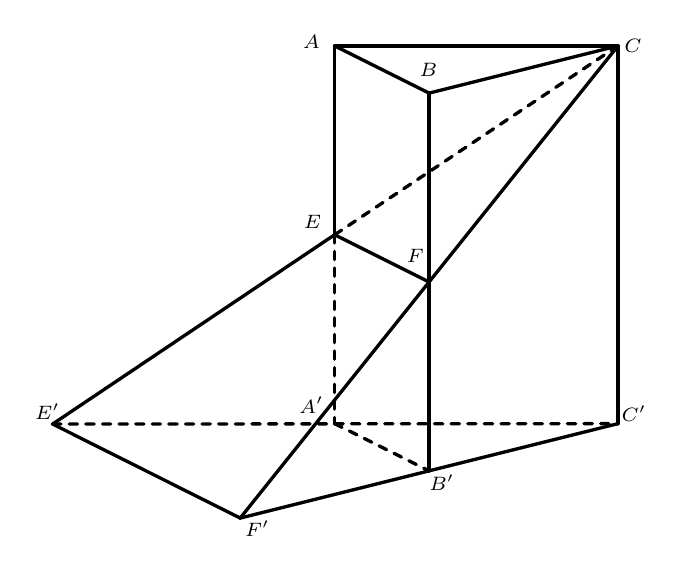
\begin{tikzpicture}[line cap=round,line join=round,>=triangle 45,x=0.012cm,y=0.012cm]
    % \clip(-688.9650857050052,-703.5746060309538) rectangle (312.48744227387573,97.82139895237928);
    \draw [line width=1.2pt] (-200.,-50.)-- (-200.,-250.);
    \draw [line width=1.2pt] (100.,-50.)-- (-200.,-50.);
    \draw [line width=1.2pt] (-100.,-100.)-- (-200.,-50.);
    \draw [line width=1.2pt] (100.,-50.)-- (-100.,-100.);
    \draw [line width=1.2pt] (-100.,-100.)-- (-100.,-300.);
    \draw [line width=1.2pt] (-100.,-500.)-- (-100.,-300.);
    \draw [line width=1.2pt] (100.,-450.)-- (-100.,-500.);
    \draw [line width=1.2pt,dash pattern=on 3pt off 3pt] (-200.,-450.)-- (-100.,-500.);
    \draw [line width=1.2pt] (100.,-450.)-- (100.,-50.);
    \draw [line width=1.2pt,dash pattern=on 3pt off 3pt] (-498.59181819578856,-450.44996720831983)-- (100.,-450.);
    \draw [line width=1.2pt,dash pattern=on 3pt off 3pt] (-200.,-250.)-- (-200.,-450.);
    \draw [line width=1.2pt] (-200.,-250.)-- (-100.,-300.);
    \draw [line width=1.2pt] (100.,-50.)-- (-100.,-300.);
    \draw [line width=1.2pt] (-300.,-550.)-- (-498.59181819578856,-450.44996720831983);
    \draw [line width=1.2pt] (-300.,-550.)-- (-100.,-300.);
    \draw [line width=1.2pt] (-300.,-550.)-- (-100.,-500.);
    \draw [line width=1.2pt,dash pattern=on 3pt off 3pt] (100.,-50.)-- (-200.,-250.);
    \draw [line width=1.2pt] (-200.,-250.)-- (-498.59181819578856,-450.44996720831983);
    \begin{scriptsize}
    \draw [fill=black] (-200.,-50.) circle (0.5pt);
    \draw[color=black] (-224.50637821947285,-45.49394500449414) node {$A$};
    \draw [fill=black] (-100.,-100.) circle (0.5pt);
    \draw[color=black] (-100.49473339965814,-75.91189555860605) node {$B$};
    \draw [fill=black] (100.,-50.) circle (0.5pt);
    \draw[color=black] (115.94068444624486,-50.173629705126736) node {$C$};
    \draw [fill=black] (-200.,-250.) circle (0.5pt);
    \draw[color=black] (-223.33645704192742,-236.19109655527265) node {$E$};
    \draw [fill=black] (-200.,-450.) circle (0.5pt);
    \draw[color=black] (-224.50637821947285,-430.3980116315256) node {$A'$};
    \draw [fill=black] (-100.,-500.) circle (0.5pt);
    \draw[color=black] (-86.45567926911309,-512.2924938925961) node {$B'$};
    \draw [fill=black] (100.,-450.) circle (0.5pt);
    \draw[color=black] (117.11060562379028,-439.7573810327908) node {$C'$};
    \draw [fill=black] (-100.,-300.) circle (0.5pt);
    \draw[color=black] (-114.53378753020321,-272.4586529851753) node {$F$};
    \draw [fill=black] (-498.59181819578856,-450.44996720831983) circle (0.5pt);
    \draw[color=black] (-504.1175396528286,-437.4175386824745) node {$E'$};
    \draw [fill=black] (-300.,-550.) circle (0.5pt);
    \draw[color=black] (-281.8325159191985,-561.4291832492385) node {$F'$};
    \end{scriptsize}
    \end{tikzpicture}
\begin{enumerate}[label=(\alph*)]
    \item Hình chóp $C.A'B'C'$ và hình lăng trụ $ABC.A'B'C'$ có đáy và đường cao bằng nhau nên $V_{C.A'B'C'} = \frac{1}{3} V$. Từ đó suy ra $V_{C.ABB'A'} = V - \frac{1}{3}V = \frac{2}{3} V$.
    
    Do $EF$ là đường trung bình của hình bình hành $ABB'A'$, nên diện tích $ABFE$ bằng nửa diện tích $ABB'A'$. Do đó $V_{C.ABFE} = \frac{1}{2} V_{C.ABB'A'} = \frac{1}{3} V$.
    
    \item Áp dụng câu a, ta có $V_{(H)} = V_{ABC.A'B'C'} - V_{C.ABFE} = V - \frac{1}{3} V = \frac{2}{3} V$.
    
    Vì $EA'$ song song và bằng $\frac{1}{2} CC'$ nên theo định lý Ta-lét, $A'$ là trung điểm của $E'C'$. Tương tự, $B'$ là trung điểm của $F'C'$. Do đó, diện tích tam giác $C'E'F'$ gấp bốn lần diện tích tam giác $A'B'C'$. Từ đó suy ra $V_{C.E'F'C'} = 4 V_{C.A'B'C'} = \frac{4}{3} V$.
    
    Do đó $\frac{V_{(H)}}{V_{C.E'F'C'}} = \frac{1}{2}$.
\end{enumerate}
\chapter*{Kết luận}
\addcontentsline{toc}{chapter}{Kết luận}

Trong nghiên cứu này, chúng tôi đã thực hiện một số phân tích quan trọng về hai chủ đề chính: mô hình nhân tố trực giao và hình học thể tích trong chương trình hình học lớp 12. Dưới đây là tổng kết về những kết quả và nhận định quan trọng:

\section*{Mô hình nhân tố trực giao}

Phần nghiên cứu về mô hình nhân tố trực giao đã cung cấp cái nhìn sâu sắc vào cấu trúc ẩn của dữ liệu và mối quan hệ giữa các biến quan sát và các nhân tố không quan sát được. Chúng tôi đã:

\begin{itemize}
    \item Xác định và mô tả cấu trúc ẩn trong dữ liệu thông qua việc áp dụng mô hình nhân tố trực giao.
    \item Sử dụng các phương pháp thống kê để đánh giá mức độ phù hợp của mô hình với dữ liệu thực tế.
    \item Phát triển kỹ thuật kiểm định giả định để đảm bảo tính chính xác của mô hình.
\end{itemize}

Kết quả cho thấy mô hình nhân tố trực giao có thể là một công cụ mạnh mẽ để hiểu sâu hơn về dữ liệu và cung cấp thông tin quan trọng cho quyết định và dự đoán.

\section*{Hình học}

Nghiên cứu về hình học thể tích lớp 12 đã đem lại những hiểu biết quan trọng về không gian ba chiều và ứng dụng của hình học trong thực tế. Chúng tôi đã:

\begin{itemize}
    \item Mô tả ý nghĩa của việc nghiên cứu về thể tích khối lăng trụ trong chương trình hình học lớp 12.
    \item Tóm tắt các khái niệm và ứng dụng của hình học thể tích trong các lĩnh vực như kiến trúc, xây dựng, và kỹ thuật.
    \item Phát triển kỹ năng giải quyết vấn đề và logic thông qua việc giải các bài toán liên quan đến thể tích khối lăng trụ.
\end{itemize}

Kết quả cho thấy việc nắm vững kiến thức về hình học thể tích là quan trọng không chỉ trong học tập mà còn trong cuộc sống và sự nghiệp sau này.

\section*{Tổng kết}

Tổng kết lại, nghiên cứu về mô hình nhân tố trực giao và hình học thể tích lớp 12 đã cung cấp cái nhìn sâu sắc vào hai chủ đề quan trọng trong toán học và hình học. Các kết quả và nhận định từ nghiên cứu này có thể đóng góp vào sự hiểu biết và ứng dụng của học thuật trong thực tiễn.

\addcontentsline{toc}{chapter}{Tài liệu tham khảo}
\begin{thebibliography}{9}
\bibitem{hinhhoc12}
Trần Văn Hạo, Nguyễn Mộng Hy, Khu Quốc Anh, Trần Đức Huyến,
{\em Hình Học 12},
Bộ Giáo Dục và Đào Tạo, 
Tái bản lần thứ mười một, 2024.
\bibitem{ttdeo}
Trịnh Thanh Đèo,
{\em Soạn thảo và chế bản tài liệu toán học với \LaTeX2$\varepsilon$},
NXB Đại~học Quốc gia TP.HCM, 2006.
\bibitem{johson}
Johnson Richard, Wichern Dean,
{\em Applied Multivariate Statistical Analysis}, tái bản lần thứ tư, Springer-Verlag, 2013.
\end{thebibliography}
% Johnson, Richard A_Wichern, Dean W - Applied Multivariate Statistical Analysis 2013
\newpage
\addcontentsline{toc}{chapter}{\indexname}
\printindex
\end{document}
